\section{Madelung treatment }
\begin{frame}
    \frametitle{Curves for 14e19o}
    \begin{figure}
        \centering
        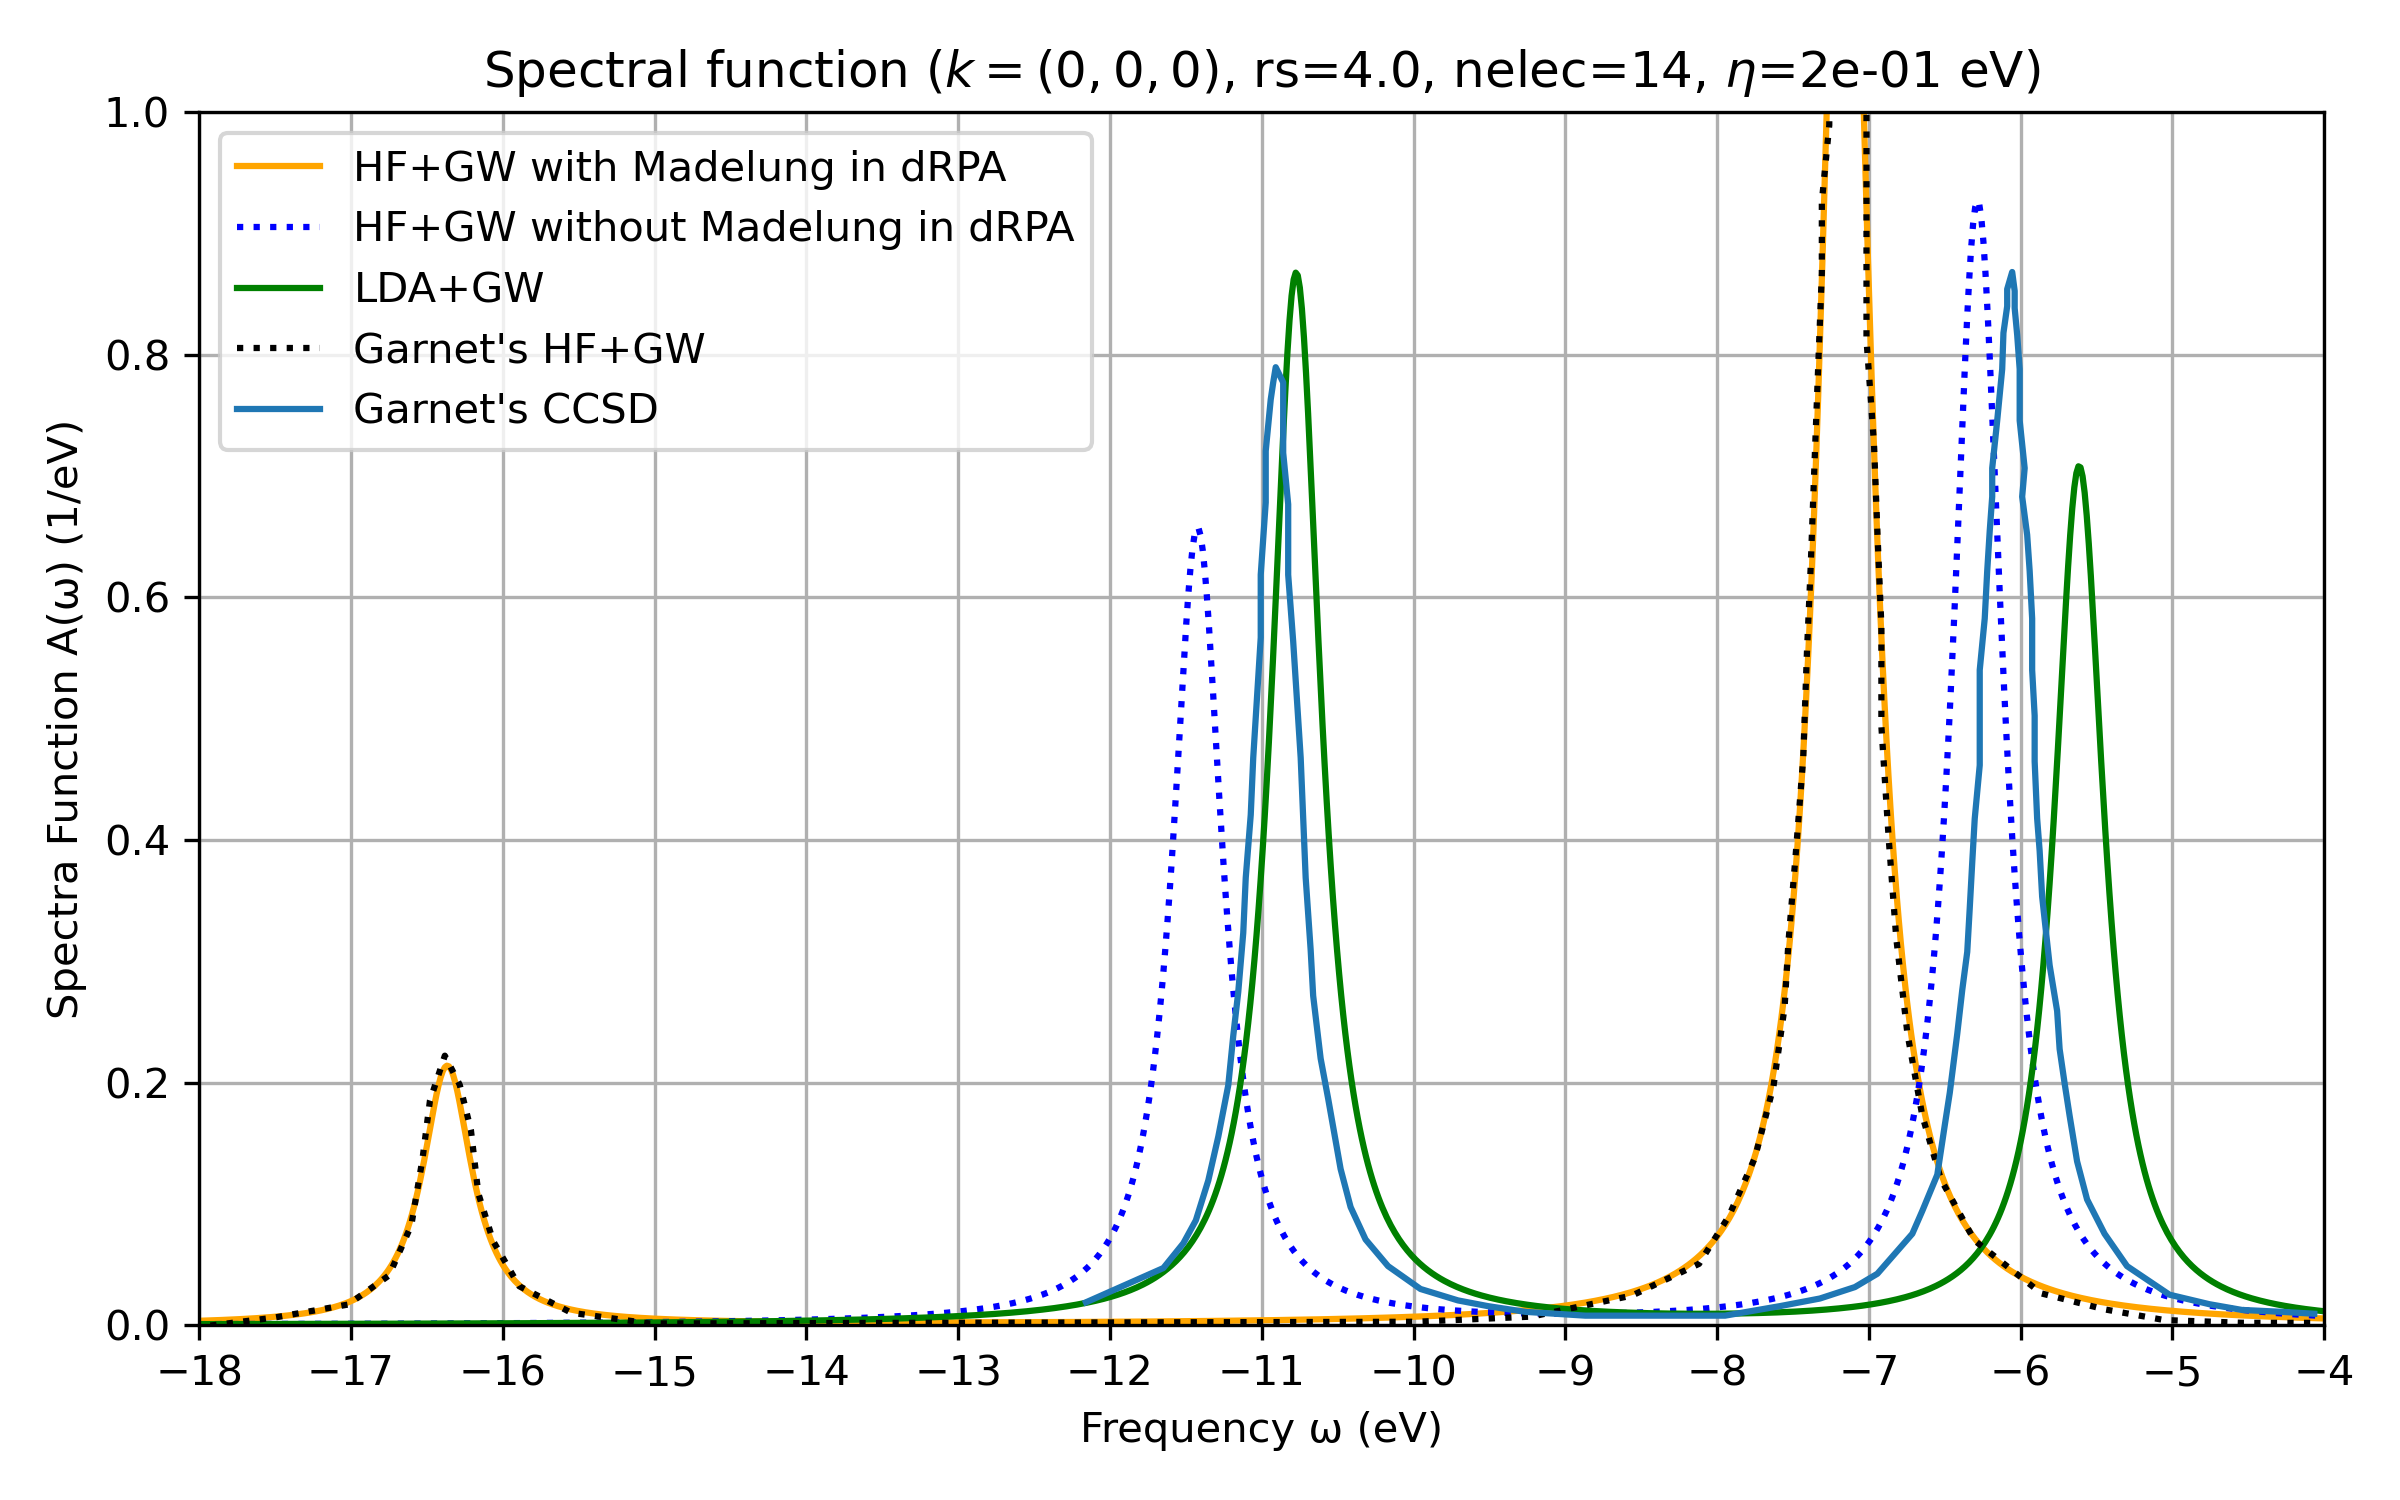
\includegraphics[width=0.8\textwidth]{26/9/9-31/image (2).png}
\end{figure}
\end{frame}
\begin{frame}
\frametitle{Why the self-energy needs unshifted HF energies: CIS}
With primes denoting Madelung-uncorrected quantities, we can rewrite normal-ordered Hamiltonian as 
\begin{equation}
    \hat H_N
    =
    \underbrace{\sum_{\mathbf{k}}\left(
    \frac{k^2}{2} - \frac{1}{\Omega}
    \sum_{\mathbf{q}\neq\mathbf{0}} v_q n_{\mathbf{k}+\mathbf{q}}
    \right) :\hat a_{\mathbf{k}}^\dagger \hat a_{\mathbf{k}}:
    +
    \hat V_{\mathrm{res}}}_{\hat H_N'}
    +
     \frac{v_M}{2} \hat N,
\end{equation}\pause
CIS writes, with $
    E_0
    \equiv
    \langle\Phi_0|\hat H_N|\Phi_0\rangle$ and $
    E_0'
    \equiv
    \langle\Phi_0|\hat H_N'|\Phi_0\rangle$
\begin{align}
    A_{ia,jb}
    &=
    \langle\Phi_i^a|
    \hat H_N-E_0
    |\Phi_j^b\rangle\\
    &=
    \left\langle\Phi_i^a\left|
    \hat H_N'
    +
    \frac{v_M}{2}\hat N
    -
    E_0'
    -
    \frac{N v_M}{2}
    \right|\Phi_j^b\right\rangle
    \\
    &=
    \langle\Phi_i^a|
    \hat H_N'-E_0'
    |\Phi_j^b\rangle
    +
    \frac{v_M}{2}
    \langle\Phi_i^a|
    \hat N-N
    |\Phi_j^b\rangle \\
&= \langle\Phi_i^a|
    \hat H_N'-E_0'
    |\Phi_j^b\rangle.
\end{align}
\end{frame}
\begin{frame}
\frametitle{Why the self-energy needs unshifted HF energies: MP2}
We agree that the MP2 correlation energy $E^{(2)}$ should be Madelung-free. \pause In BWs2, we need $\operatorname{Tr}(\mathbf{W}^{O}) - \operatorname{Tr}(\mathbf{W}^{V}) = E^{(2)}$. \pause But
\begin{align}
{W}^{O}_{ii} &\equiv \frac{1}{2}\bm{\Sigma}_{ii}^{(2),2p1h}[\hat F](\omega = \epsilon_i^{\rm HF}) = \frac{1}{2}\sum_{a b j} \frac{\mathcal{K}_{ij}^{ab}}{\epsilon^{\rm HF}_i + \epsilon^{\rm HF}_j - \epsilon^{\rm HF}_a - \epsilon^{\rm HF}_b}\\
&= \frac{1}{2}\bm{\Sigma}_{ii}^{(2),2p1h}[\hat F'](\omega = \epsilon'^{\rm HF}_i) =\frac{1}{2}\sum_{a b j} \frac{\mathcal{K}_{ij}^{ab}}{\epsilon'^{\rm HF}_i + \epsilon'^{\rm HF}_j - \epsilon'^{\rm HF}_a - \epsilon'^{\rm HF}_b},\\
{W}^{V}_{aa} &\equiv \frac{1}{2}\bm{\Sigma}_{aa}^{(2),2h1p}[\hat F](\omega = \epsilon^{\rm HF}_a)= \frac{1}{2}\sum_{i j b} \frac{\mathcal{K}_{ij}^{ab}}{\epsilon^{\rm HF}_a + \epsilon^{\rm HF}_b - \epsilon^{\rm HF}_i - \epsilon^{\rm HF}_j}\\
&= \frac{1}{2}\bm{\Sigma}_{aa}^{(2),2h1p}[\hat F'](\omega = \epsilon'^{\rm HF}_a) = \frac{1}{2}\sum_{i j b} \frac{\mathcal{K}_{ij}^{ab}}{\epsilon'^{\rm HF}_a + \epsilon'^{\rm HF}_b - \epsilon'^{\rm HF}_i - \epsilon'^{\rm HF}_j}.
\end{align}
\end{frame}
\begin{frame}
\frametitle{Why the self-energy needs unshifted HF energies: MP2}
\begin{align}
  \Sigma^{(2)}[F](\omega)&\equiv \bm{\Sigma}^{(2),2p1h}[F](\omega) + \bm{\Sigma}^{(2),2h1p}[F](\omega)  \\
&= \sum_{ia b} \frac{\mathcal{K}_{pi}^{ab}}{\omega - \epsilon^{\rm HF}_a - (\epsilon^{\rm HF}_b-\epsilon^{\rm HF}_i)} + \sum_{i j a} \frac{\mathcal{K}_{ij}^{pa}}{\omega-\epsilon^{\rm HF}_i + (\epsilon^{\rm HF}_a - \epsilon^{\rm HF}_j)}\\
&= \sum_{ia b} \frac{\mathcal{K}_{pi}^{ab}}{\omega' - \epsilon'^{\rm HF}_a - (\epsilon'^{\rm HF}_b-\epsilon'^{\rm HF}_i)} + \sum_{i j a} \frac{\mathcal{K}_{ij}^{pa}}{\omega'-\epsilon'^{\rm HF}_i + (\epsilon'^{\rm HF}_a - \epsilon'^{\rm HF}_j)}\label{eq:second_order_self_energy}\\
&\equiv \bm{\Sigma}^{(2),2p1h}[F'](\omega') + \bm{\Sigma}^{(2),2h1p}[F'](\omega'),
\end{align}
where $\omega' = \omega - \frac{v_M}{2}$. \pause The following quasiparticle equations are the same
\begin{align}
\omega - \epsilon^{\rm HF}_p - \bm{\Sigma}^{(2)}_{pp}[\hat F](\omega) &= 0\\
\omega' - \epsilon'^{\rm HF}_p - \bm{\Sigma}^{(2)}_{pp}[\hat F'](\omega') &= 0
\end{align} 
\end{frame}
\begin{frame}
\frametitle{Conclusion}
What to do for one-shot spectral functions? 
\begin{enumerate}
    \item Evaluate the QP equation with a uniform shift of $+\frac{v_M}{2}$ to occupied and virtuals. \pause
    \item Shift IPs and EAs by $-\frac{v_M}{2}$ on physical spectral functions. \pause
    \item Items 1 and 2 have the net effect of shifting IPs by $-v_M$ and EAs by $0$. \pause
\end{enumerate}
What to do for self-consistent spectral functions? 
\begin{enumerate}
    \item Iterate on physical electron-removal and electron-addition spectral functions shifted by $-\frac{v_M}{2}$ and $+\frac{v_M}{2}$, respectively.
    \end{enumerate}
\end{frame}
\section{Derivation of the quasiboson Hamiltonian }
\begin{frame}
    \frametitle{The goal}
With $\epsilon_{\mathbf k}^{(0)}=\frac{k^2}{2}+\frac{v_M}{2}$ and $v_M=-2.837297 \times\left(\frac{3}{4 \pi}\right)^{1 / 3} N^{-1 / 3} r_s^{-1}$
\begin{align}
\hat H
&=
\sum_{\mathbf k}\epsilon_{\mathbf k}^{(0)}\hat a_{\mathbf k}^\dagger \hat a_{\mathbf k}
+
{\frac{1}{2\Omega}
\sum_{\mathbf q\neq\mathbf 0}v_q
\sum_{\mathbf k\mathbf k'}
a_{\mathbf{k}+\mathbf q}^\dagger
a_{\mathbf{k}'-\mathbf q}^\dagger
a_{\mathbf k'}
a_{\mathbf k}}\\
&=
E_{\rm HF}
+
{\sum_{\mathbf k}
\epsilon_{\mathbf k}^{\rm HF}
:
\hat a_{\mathbf k}^\dagger \hat a_{\mathbf k}
:}
+
\frac{1}{2\Omega}
\sum_{\mathbf q\neq\mathbf 0}v_q
\sum_{\mathbf k\mathbf k'}:
a_{\mathbf{k}+\mathbf q}^\dagger
a_{\mathbf{k}'-\mathbf q}^\dagger
a_{\mathbf k'}
a_{\mathbf k}:
\end{align}
where ${
\epsilon_{\mathbf k}^{\rm HF}
}
=
\frac{k^2}{2}
+
\frac{v_M}{2}
-
\frac{1}{\Omega}
\sum_{\mathbf q\neq\mathbf 0}
v_q n_{\mathbf{k}+\mathbf q}
$. \pause We want to get to 
\begin{equation}
    \hat H_{\rm eb}
    =
    -\sum_{\mathbf k\in\mathcal O}
    \epsilon_{\mathbf k}^{\rm HF}
    h_{\mathbf k}^{\dagger}h_{\mathbf k}
    +
    \sum_{\nu_{\mathbf q}}
    \omega_{\nu_{\mathbf q}}^{\rm pl}
    \hat\beta_{\nu_{\mathbf q}}^{\dagger}
    \hat\beta_{\nu_{\mathbf q}}
    +
    \sum_{\mathbf k\mathbf q}
    \sum_{\nu_{\mathbf q}}
    g_{\nu}^{\rm pl}(\mathbf k,\mathbf q)
    h_{\mathbf k+\mathbf q}^{\dagger}
    h_{\mathbf k}
    \left(
        \hat\beta_{\nu_{\mathbf q}}
        +
        \hat\beta_{\nu_{-\mathbf q}}^{\dagger}
    \right).
\end{equation}
\end{frame}
\begin{frame}
    \frametitle{Quadratic bosonic bath}
Define  $
    E_{i\mathbf q}^{\dagger}
    =
    a_{\mathbf{i}+\mathbf q}^{\dagger}a_{\mathbf i}$ and $
    E_{i\mathbf -q}
    =
    a_{\mathbf i}^{\dagger}a_{\mathbf{i}-\mathbf q}$ with $\hat\kappa[\mathbf z]
    =
    \sum_{i\mathbf q}
    \left[
        \kappa_{i\mathbf q}
        E_{i\mathbf q}^{\dagger}
        -
        \kappa_{i\mathbf q}^{*}
        E_{i\mathbf q}
    \right]$ using $
    \boldsymbol{\kappa}_{\mathbf q}
    =
    \begin{pmatrix}
        \kappa_{1\mathbf q}\\
        \kappa_{2\mathbf q}\\
        \vdots
    \end{pmatrix}
$ and $
    {
    \mathbf z_{\mathbf q}
    =
    \begin{pmatrix}
        \boldsymbol{\kappa}_{\mathbf q}\\
        \boldsymbol{\kappa}_{-\mathbf q}^{*}
    \end{pmatrix}
    }
$. \pause Given $    |\Phi(\mathbf z)\rangle
    =
    e^{\hat\kappa[\mathbf z]}
    |\Phi_0\rangle$, we have \begin{align}
    E(\mathbf z)
    &=
    \langle\Phi(\mathbf z)|
    \hat H
    |\Phi(\mathbf z)\rangle
    \\
    % &=
    % \langle\Phi_0|
    % e^{-\hat\kappa[\mathbf z]}
    % \hat H
    % e^{\hat\kappa[\mathbf z]}
    % |\Phi_0\rangle\\
    &=
    E_{\rm HF}
    +
    \langle\Phi_0|
    [\hat H,\hat\kappa[\mathbf z]]
    |\Phi_0\rangle
+
    \frac{1}{2}
    \langle\Phi_0|
    [[\hat H,\hat\kappa[\mathbf z]],\hat\kappa[\mathbf z]]
    |\Phi_0\rangle
    +
    \ldots \\ 
\implies     \nabla_{\mathbf z}E(\mathbf z)
    &=
    \begin{pmatrix}
        \dfrac{\partial E(\mathbf z)}
        {\partial\boldsymbol{\kappa}}\\
        \\
        \dfrac{\partial E(\mathbf z)}
        {\partial\boldsymbol{\kappa}^{*}}
    \end{pmatrix} \implies    \left.
    \nabla_{\mathbf z}E(\mathbf z)
    \right|_{\mathbf z=0}
    =
    0
    \label{eq:energy_expansion_kappa}
\end{align}
\end{frame}
\begin{frame}
    \frametitle{Quadratic bosonic bath cont.}
\begin{align}
    \mathcal H_{\rm HF}
    =
    \left.
    \frac{\partial^2 E(\mathbf z)}
    {\partial
    \begin{pmatrix}
        \boldsymbol{\kappa}^{*}\\
        \boldsymbol{\kappa}
    \end{pmatrix}
    \partial
    \begin{pmatrix}
        \boldsymbol{\kappa}&
        \boldsymbol{\kappa}^{*}
    \end{pmatrix}}
    \right|_{\mathbf z=0}
    &={
    \begin{pmatrix}
        A & B\\
        B^{*} & A^{*}
    \end{pmatrix}.
    }
\end{align} \pause
Thus, the second-order correction to the HF energy is
\begin{align}
E^{(2)}(\mathbf \kappa, \mathbf \kappa^{*})
    &=
    \frac{1}{2}
    \begin{pmatrix}
        \boldsymbol{\kappa}_{\mathbf q}^{*} &
        \boldsymbol{\kappa}_{-\mathbf q}
    \end{pmatrix}
    \begin{pmatrix}
        A & B\\
        B^{*} & A^{*}
    \end{pmatrix}
    \begin{pmatrix}
        \boldsymbol{\kappa}_{\mathbf q}\\
        \boldsymbol{\kappa}_{-\mathbf q}^{*}
    \end{pmatrix}
\end{align}\pause
Quantizing the space and then applying Bogoliubov transformation gives 
\begin{align}
    \hat{H}^{(2)}&= \frac{1}{2}
    \begin{pmatrix}
        \hat{\bm{b}}_{\mathbf q}^{\dagger} &
        \hat{\bm{b}}_{-\mathbf q}
    \end{pmatrix}
    \begin{pmatrix}
        A & B\\
        B^{*} & A^{*}
    \end{pmatrix}
    \begin{pmatrix}
        \hat{\bm{b}}_{\mathbf q}\\
        \hat{\bm{b}}_{-\mathbf q}^{\dagger}
    \end{pmatrix}\\
    &=
    \hat{\bm{\beta}}_{\mathbf q}^{\dagger} \boldsymbol{\Omega}_{\mathbf q} \hat{\bm{\beta}}_{\mathbf q}
    +
    \frac{1}{2}\operatorname{Tr}(\boldsymbol{\Omega}_{\mathbf q}-A)+\frac{1}{2}\operatorname{Tr}(A)\\
&= \sum_{\nu_{\mathbf q}} \omega_{\nu_{\mathbf q}} \hat{\beta}_{\nu_{\mathbf q}}^{\dagger} \hat{\beta}_{\nu_{\mathbf q}} + E_{\rm RPA} + \frac{1}{2}\operatorname{Tr}(A)
\end{align}
\end{frame}
\begin{frame}
    \frametitle{Pure fermionic and coupling terms}
Start with 
\begin{equation}
    \hat H_{\rm h}(\boldsymbol{\kappa})
    =
    \sum_{\mathbf k,\mathbf k'\in\mathcal O}
    h^{\rm h}_{\mathbf k'\mathbf k}(\boldsymbol{\kappa})
    h_{\mathbf k'}^\dagger h_{\mathbf k}.
    \label{eq:hole_hamiltonian_kappa}
\end{equation} \pause Expand to first order about the
Hartree--Fock reference
\begin{align}
    h^{\rm h}_{\mathbf k'\mathbf k}(\boldsymbol{\kappa})
    &=
    h^{\rm h}_{\mathbf k'\mathbf k}(0)+
    \sum_{i\mathbf q}
    \left.
    \frac{\partial
    h^{\rm h}_{\mathbf k'\mathbf k}}
    {\partial\kappa_{i\mathbf q}}
    \right|_{0}
    \kappa_{i\mathbf q}+
    \sum_{i\mathbf q}
    \left.
    \frac{\partial
    h^{\rm h}_{\mathbf k'\mathbf k}}
    {\partial\kappa_{i\mathbf q}^{*}}
    \right|_{0}
    \kappa_{i\mathbf q}^{*}
    +
    \mathcal O(\kappa^2),
    \label{eq:hole_hamiltonian_expansion}
\end{align} 
\pause
\begin{align}
    \left.
    \frac{\partial
    h^{\rm h}_{\mathbf k+\mathbf q,\mathbf k}}
    {\partial\kappa_{i\mathbf q}}
    \right|_0
    &=
    -
    \left.
    \frac{\partial
    F_{\mathbf k,\mathbf k+\mathbf q}}
    {\partial\kappa_{i\mathbf q}}
    \right|_0
    \\
    &=
    -
    \sum_{\mathbf l}
    \frac{\partial
    F_{\mathbf k,\mathbf k+\mathbf q}}
    {\partial P_{\mathbf l + \mathbf q,\mathbf l}}
    \left.
    \frac{\partial
    P_{\mathbf l + \mathbf q,\mathbf l}}
    {\partial\kappa_{i\mathbf q}}
    \right|_0 \\
&= 
    -
\frac{v(\mathbf q)}{\Omega} \sum_{\mathbf l}
    \delta_{\mathbf l,\mathbf i}
\end{align}
\end{frame}
\begin{frame}
    \frametitle{Pure fermionic and coupling terms cont.}
So up to linear order in $\boldsymbol{\kappa}$
\begin{align}
    \hat H_{\rm h}(\boldsymbol{\kappa})
    &\overset{\text{direct}}{=} -
    \sum_{\mathbf k\in\mathcal O}
    \epsilon_{\mathbf k}^{\rm HF}
    h_{\mathbf k}^{\dagger}h_{\mathbf k}
-
    \sum_{\mathbf k\mathbf q}
    \sum_i
    \frac{v(\mathbf q)}{\Omega}
    h_{\mathbf k+\mathbf q}^{\dagger}h_{\mathbf k}
    \left(
        \kappa_{i\mathbf q}
        +
        \kappa_{i,-\mathbf q}^{*}
    \right)
    \label{eq:hole_hamiltonian_linear_kappa}
\end{align} \pause
Quantizing again and then applying the Bogoliubov transformation gives
\begin{align}
    \hat H_{\rm h-pl}
    &=
    \sum_{\mathbf k\mathbf q}
    \sum_{\nu_{\mathbf q}}
    g_{\nu}^{\rm pl}(\mathbf k,\mathbf q)
    h_{\mathbf k+\mathbf q}^{\dagger}
    h_{\mathbf k}
    \left(
        \hat\beta_{\nu_{\mathbf q}}
        +
        \hat\beta_{\nu_{-\mathbf q}}^{\dagger}
    \right),
    \label{eq:hole_plasmon_coupling}
\end{align} \pause
with
\begin{equation}
    {
    g_{\nu}^{\rm pl}(\mathbf k,\mathbf q)
    =
    -\frac{v(\mathbf q)}{\Omega}
    \sum_{\mathbf i}
    \left[
        X_{i\nu}(\mathbf q)
        +
        Y_{i\nu}(\mathbf q)
    \right].
    }
    \label{eq:screened_hole_plasmon_coupling}
\end{equation}\pause
So overall (omitting constant terms)
\begin{equation}
    \hat H_{\rm eb}
    =
    -\sum_{\mathbf k\in\mathcal O}
    \epsilon_{\mathbf k}^{\rm HF}
    h_{\mathbf k}^{\dagger}h_{\mathbf k}
    +
    \sum_{\nu_{\mathbf q}}
    \omega_{\nu_{\mathbf q}}^{\rm pl}
    \hat\beta_{\nu_{\mathbf q}}^{\dagger}
    \hat\beta_{\nu_{\mathbf q}}
    +
    \sum_{\mathbf k\mathbf q}
    \sum_{\nu_{\mathbf q}}
    g_{\nu}^{\rm pl}(\mathbf k,\mathbf q)
    h_{\mathbf k+\mathbf q}^{\dagger}
    h_{\mathbf k}
    \left(
        \hat\beta_{\nu_{\mathbf q}}
        +
        \hat\beta_{\nu_{-\mathbf q}}^{\dagger}
    \right).
\end{equation}


\end{frame}
